
\documentclass[fleqn,addpoints]{exam}
\usepackage{amsmath}
\usepackage{graphicx}
\usepackage{float}
\usepackage{caption}
\usepackage{polynom}
\usepackage{mdwlist}

\printanswers

\ifprintanswers
\usepackage{2in1, lscape}
\fi

\title{Math 115 Chapter Three Exam}
\date{April 19, 2011}

\author{}

\begin{document}

\maketitle  

\ifprintanswers
\else
\vspace{0.2in}
\makebox[\textwidth]{Name:\enspace\hrulefill}
\vspace{0.2in}

\begin{center}
\gradetable[h][pages]
% \bonusgradetable[h][pages]
\end{center}

\else

\section{Instructions}

Calculators aren't allowed on the final, so they also aren't allowed on any other tests.  If the answer involves a
logarithm or exponential, just leave the answer as $\dfrac{\ln 7}{2}$ (or whatever it is).

\fi

\section{Evaluation} 
 
For questions 1 to \ref{evaluate:last}, evaluate each expression.
 
\begin{questions}
\label{evaluate:first}
\question[3]
\[
  \log_4 64
\]
\begin{solution}[2 cm]
\[
  \log_4 64 = \log_4 4^3 = 3
\]

\end{solution}

% \question[7]
% \[
%   \log_7 \sqrt[4]{49}
% \]
% \begin{solution}[1.5 cm]
% \end{solution}

\question[7]
\label{evaluate:last}
\[
  \log_9 3 + \log_9 27
\]
\begin{solution}[3 cm]
\[
  \log_9 3 + \log_9 27 = \log_9 (3 \cdot 27) = \log_9 81 = \log_9 9^2 = 2
\]
\end{solution}

\ifprintanswers
\else
\pagebreak
\fi


\section{Graphing}


\question[10]
Find the domain, intercepts, and asymptotes and sketch the graph of $f(x)$. 

\label{graph:first}
\[
  f(x) = \log_2 (x-2) 
\]

\begin{solution}[5 cm]
\begin{itemize}
\item domain: $x > 2$
\item x-intercept: (3, 0)
\item no y-intercept
\item vertical asymptote: $x=2$
\end{itemize}

\begin{figure}[H]
  \centering
  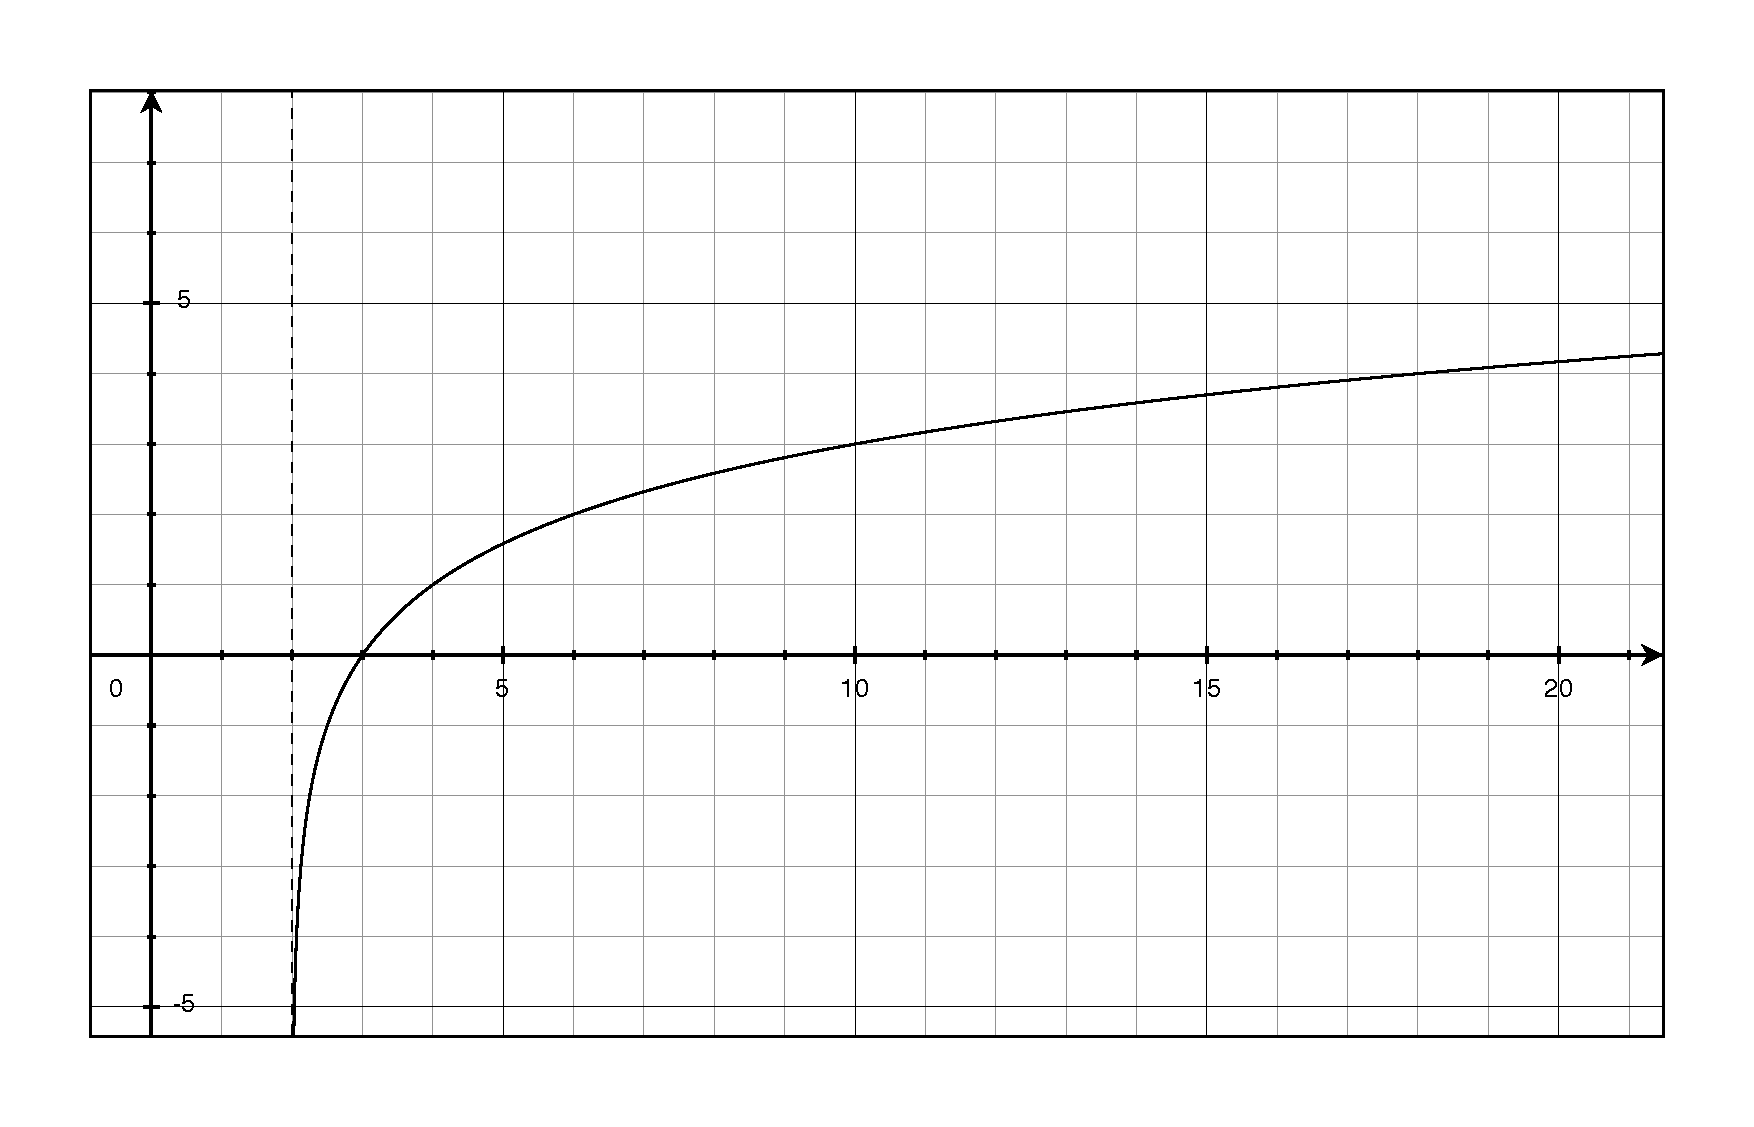
\includegraphics[scale=.3]{graph_solution.eps}
  \caption*{Question \ref{graph:first}}
\end{figure}

\end{solution}

\ifprintanswers
\else
\begin{figure}[H]
  \centering
  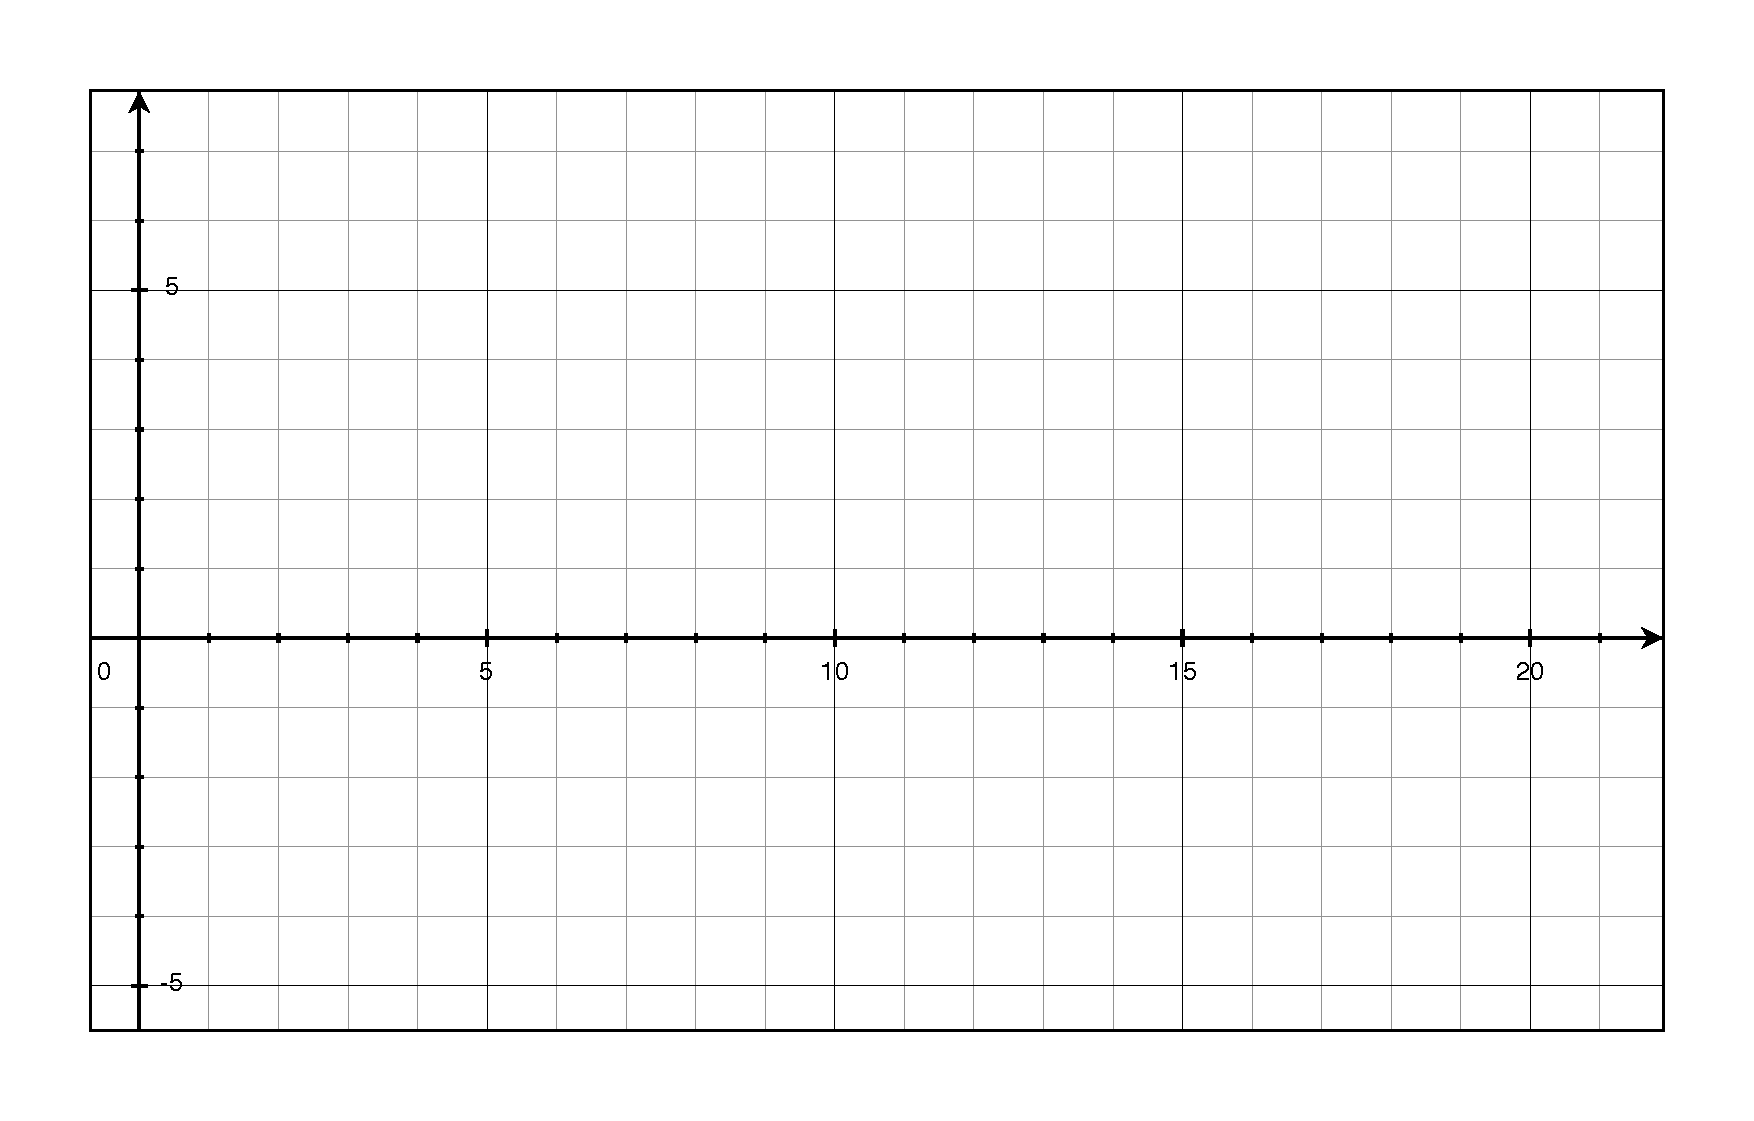
\includegraphics[scale=.6]{graph1.eps}
  \caption*{Question \ref{graph:first}}
\end{figure}
\fi

\pagebreak

\section{Change of Base}
\question[3]
Write as a ratio of logarithms.
\[
  \log_5 7
\]
\begin{solution}[1 cm]
\[
  \log_5 7 = \frac{\ln 7}{\ln 5}
\]
\end{solution}

\question[2]
Write as a single logarithm (in a different base).
\[
  \frac{\ln 3}{\ln 2}
\]
\begin{solution}[1 cm]
\[
  \frac{\ln 3}{\ln 2} = \log_2 3
\]
\end{solution}

\section{Transformations}

For questions \ref{transform:first} to \ref{transform:last}, expand to the sum, difference, and/or constant multiple of
logarithms. 

\question[3]
\label{transform:first}
\[
  \ln xyz
\]
\begin{solution}[3 cm]
\[
  \ln xyz = \ln x + \ln y + \ln z
\]
\end{solution}

\question[7]
\[
  \log \frac{ \sqrt{xy} } { z } 
\]
\begin{solution}[4 cm]
\begin{align*}
  \log \frac{ \sqrt{xy} } { z } &= \frac{1}{2} \log xy - \log z \\
  &= \frac{1}{2} (\log x + \log y) - \log z
\end{align*}

\end{solution}

\ifprintanswers
\else
\pagebreak
\fi

\question[10]
\label{transform:last}
\[
  \log \frac{x}{y(x^2-2)^{1/3}} 
\]
\begin{solution}[4 cm]
\begin{align*}
  \log \frac{x}{y(x^2-2)^{1/3}} &= \log x - \log \left[ y(x^2-2)^{1/3} \right] \\
  &= \log x - \left[ \log y + \log(x^2-2)^{1/3} \right] \\
  &= \log x - \log y - \log(x^2-2)^{1/3} \\
  &= \log x - \log y - \frac{1}{3}\log(x^2-2) \\
\end{align*}
\end{solution}

For questions \ref{condense:first} to \ref{condense:last}, condense to the logarithm of a single quantity.

\question[5]
\label{condense:first}
\[
  \ln x + 2 \ln y
\]
\begin{solution}[3 cm]
\[
  \ln x + 2 \ln y = \ln xy^2
\]

\end{solution}

\question[7]
\[
  \ln x - \frac{1}{2} \ln y + \ln z
\]
\begin{solution}[4 cm]
\begin{align*}
  \ln x - \frac{1}{2} \ln y + \ln z &= \ln x - \ln y^{1/2} + \ln z  \\
  &= \ln x + \ln z - \ln y^{1/2}   \\
  &= \ln xz - \ln y^{1/2}   \\
  &= \ln \frac{xz}{y^{1/2}} \\
\end{align*}
\end{solution}

\question[8]
\label{condense:last}
\[
  2 \log x - \frac{1}{3} \log (x^2 + 5)
\]
\begin{solution}[4 cm]
\[
  2 \log x - \frac{1}{3} \log (x^2 + 5) = \log \frac{x^2}{(x^2+5)^{1/3}}
\]
\end{solution}

\ifprintanswers
\else
\pagebreak
\fi

\section{Equations}

For questions \ref{equation:first} to \ref{equation:last}, solve for $x$:

\question[5]
\label{equation:first}
\[
  \log(x+3) = 1
\]
\begin{solution}[2 cm]

\begin{align*}
  \log(x+3) &= 1 \\
  x + 3 &= 10 \\
  x &= 7 \\
\end{align*}

\end{solution}

\question[7]
\[
  \log x + \log (x-1) = \log 4x
\]
\begin{solution}[3 cm]
\begin{align*}
  \log x + \log (x-1) &= \log 4x \\
  \log x(x-1) &= \log 4x \\
  x(x-1) &= 4x \\
  x^2-x &= 4x \\
  x^2-5x &= 0 \\
  x(x-5) &= 0 \\
\end{align*}

$x=5$ or $x=0$, but 0 is not in the domain of the original equation, so $x=5$ is the only solution.

\end{solution}

\question[8]
\[ 
  \frac{8}{2+e^{-x}} = 1
\]
\begin{solution}[4 cm]
\begin{align*}
  2+e^{-x} &= 8 \\ 
  e^{-x} &= 6 \\
  -x &= \ln 6 \\
  x &= -\ln 6 \\
\end{align*}

\end{solution}

\question[10]
\label{equation:last}
\[
  e^{2x} - e^x - 6 = 0
\]
\begin{solution}[4 cm]
\begin{align*}
  e^{2x} - e^x - 6 &= 0 \\
  (e^x - 3)(e^x + 2) &= 0 \\
\end{align*}

$e^x = 3$ or $e^x = -2$.  $e^x = -2$ doesn't have a real solution, so the only solution is $x = \ln 3$.

\end{solution}

\pagebreak

\section{Exponential Models}

\question[10]
The velocity of a parachuter $t$ seconds after jumping is given by $v(t) = 80(1 - e^{-0.2t})$.  After how many seconds
is the velocity 50 ft/s?

\begin{solution}[8 cm]

\begin{align*}
  50 &= 80(1 - e^{-0.2t}) \\
  50 &= 80 - 80e^{-0.2t} \\
  - 30 &= -80 e^{-0.2t} \\
  \frac{3}{8} &= e^{-0.2t} \\
  \ln \frac{3}{8} &= -0.2t \\
  \ln \frac{3}{8} &= -\frac{t}{5} \\
  t &= -5 \ln \frac{3}{8} \\
\end{align*}
\end{solution}

\ifprintanswers
\pagebreak
\fi

\question[10]
The formula for compound interest is: $A = P e^{rt}$.  Use this formula to find a function $f(t)$ which provides the
rate required to make the principal triple in $t$ years.

\begin{solution}[7 cm]
\begin{align*}
  3P &= P e^{rt} \\
  3 &= e^{rt} \\
  \ln 3 &= rt \\
  r &= \frac{\ln 3}{t} \\
  f(t) &= \frac{\ln 3}{t} \\
\end{align*}
\end{solution}

% \question[10]
% Remember that for the formula for the rate of decay element with a half life of $t_h$ remaining after $t$ years is: 
% \[
%   r = \frac{\ln 2}{t_h}
% \]

% If 30\% of the original amount of a sample of an element with a half life of 1,000 years is remaining, how old is the sample?

% \begin{solution}[5 cm]
% \end{solution}
 
\ifprintanswers
\else
\pagebreak
\fi

\section{Extra Credit}
\bonusquestion[10]

We used the equations:
\begin{align*}
  A &= A_0 e^{-rt} \\
  r &= \dfrac{\ln 2}{t_h}
\end{align*}

to compute radioactive decay.  

Another equation which says the same thing is:

\[
  A = A_0 \cdot 2^{-t/t_h}
\]

Show that this equation is equivalent to the other two equations.

\begin{solution}[5 cm]
We want to show that $A_0 e^{-t \cdot \ln 2/t_h} = A_0 \cdot 2^{-t/t_h}$:

\begin{align*}
  A_0 e^{-t (\ln 2/t_h)} &= A_0 e^{\ln 2 (-t/th)}  \\
  &= A_0 \left( e^{\ln 2} \right)^{-t/th}  \\
  &= A_0 \cdot 2^{-t/th}  \\
\end{align*}

Another way to see that the equations are equivalent is to use the definition of half-life:

\begin{align*}
  A_1 &= \frac{1}{2} A_0 \\
  A_2 &= \frac{1}{2} A_1 = \frac{1}{4} A_0 \\
  A_3 &= \frac{1}{2} A_2 = \frac{1}{8} A_0 \\
  \vdots \\
  A_n &= \frac{1}{2} A_{n-1} = \frac{1}{2^n} A_0 = A_0 \cdot 2^{-n} \\
\end{align*}

$n$ in this equation is the number of half-lives that have elapsed.  We want the time in years, not half-lives, however,
and the number of years is given by: $t = nt_h$.  If we solve for $n$ and plug the result into
the equation for $A_n$, we get: 
\[
  A_n = A_0 \cdot 2^{-t/t_h}
\]
 
\end{solution}

\end{questions}

\end{document}
